%%%%%%%%%%%%%%%%%%%% author.tex %%%%%%%%%%%%%%%%%%%%%%%%%%%%%%%%%%%
%
% sample root file for your "contribution" to a contributed volume
%
% Use this file as a template for your own input.
%
%%%%%%%%%%%%%%%% Springer %%%%%%%%%%%%%%%%%%%%%%%%%%%%%%%%%%%%%%%%%

\title{Introduction and SimCenter Goals}
% Use \titlerunning{Short Title} for an abbreviated version of
% your contribution title if the original one is too long
\author{
    \textbf{Sanjay Govindjee}
    \and Gregory G. Deierlein
    \and Frank McKenna}
\tocauthor{}
\authorrunning{Govindjee et al.}
% Use \authorrunning{Short Title} for an abbreviated version of
% your contribution title if the original one is too long
%\institute{Name of First Author \at Name, Address of Institute, %\email{name@email.address}
%\and Name of Second Author \at Name, Address of Institute %\email{name@email.address}}
%
% Use the package "url.sty" to avoid
% problems with special characters
% used in your e-mail or web address
%
\maketitle

Computational simulation is as an essential component of natural hazards engineering research and practice to assess and mitigate the damaging effects of earthquakes, wind storms and associated tsunami, and storm surge effects on communities. Recognizing the challenge as broad and multi-disciplinary, and encompassing natural hazards across a wide range of scales, the SimCenter's approach is to leverage existing software platforms by creating computational workflow technologies that can seamlessly integrate a broad array of simulation software with high-performance computing platforms and data repositories. In addition to developing and releasing the computational workflow tools and training modules, the SimCenter is engaging with researchers to extend the simulation capabilities through collaboration with NHERI researchers. Collaboration opportunities range from facilitating research on application testbed studies to implementation of new computational formulations.

The SimCenter is creating workflow tools that range from ones that enable the study of the response of single buildings given a natural hazard event to others that perform end-to-end simulations of natural hazard effects on communities. An important emphasis of the workflows are capabilities to incorporate and propagate inherent variabilities and modeling uncertainties through the computational simulations. Another focus is on tools to develop datasets and integrate them with the computational tools, with particular emphasis on data and simulation software available on the NHERI DesignSafe platform.

To a large extent, the most distinguishing innovation of the SimCenter simulation tools are to provide a computational ecosystem that will enable the NHERI research community to achieve unprecedented capabilities to conduct end-to-end simulations. By employing an open-source framework, the ecosystem will allow researchers to contribute to some or all aspects of the simulation capabilities. The overall concept is illustrated in Figure \ref{fig:intro_CompFramework}, where the challenge is to link models and data from descriptions of the assets (buildings, bridges, civil infrastructure, and other components of the built environment), hazard effects (earthquake ground motions, wind, water inundation), through to effects on the assets and implications on community function and recovery. The SimCenter computational and data tools lie at the heart of the simulation, linking upstream data from natural hazard models to downstream socio-economic outcomes and models of communities. Figure \ref{fig:intro_CompFramework} illustrates where four SimCenter tools (uqFEM, EE-UQ, CWE-UQ, and PBE) fit into the computational workflow. Underlying these tools are software applications that can be incorporated in specific tools (with graphical user interfaces) or incorporated in workflow scripts that are more fluid and adaptable to alternative regional hazard scenario simulations. 

\begin{figure}[htb]
    \centering
    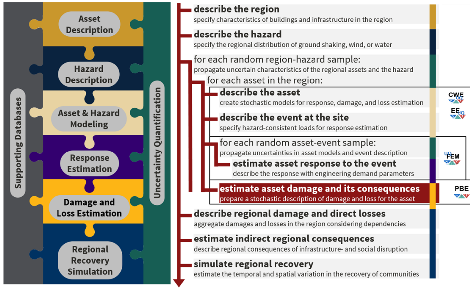
\includegraphics[width=1.0\textwidth, angle = 0]{editor/Figures/CompFramework.pdf}
    \caption{Computational framework for end-to-end simulations of natural hazard effects on damage and recovery of the built environment and communities}
    \label{fig:intro_CompFramework}
\end{figure}

The following is a summary of computational workflow implementations that the SimCenter is actively working on and has either already deployed or will deploy in the immediate future:

\paragraph{uqFEM} The uqFEM application facilitates uncertainty quantification, model calibration, optimization and sensitivity analyses of structural and geotechnical materials, components, and systems by combining existing finite element applications with uncertainty quantification (UQ) application. The V1.1.0 release links two finite-element codes (OpenSEES or FEAPpv) with uncertainty quantification functions in DAKOTA. A graphical user interface is provided with basic functionality to define random variables in the finite-element models and invoke certain UQ methods from DAKOTA. Running through the HPC capabilities of DesignSafe, or on a user's desktop computer, the system makes available unprecedented capabilities for natural hazards researchers to perform UQ simulations. Future plans include extensions to include links to other finite element codes that are running on DesignSafe (e.g., LSDyna) and uncertainty quantification toolboxes (UQ-Pyt, UQpy).
%\newline

\paragraph{CWE-UQ} The Computational Wind Engineering (CWE) Tool is an application to simulate the response of structures to wind forces. The V2.0 release of the tool will allow users to select from a variety of options for specifying wind forces on structures from stochastic loading models and online wind engineering databases through to performing computationally intense Computational Fluid Dynamics (CFD) analysis utilizing applications such as OpenFOAM. The tool is intended to make detailed CFD modeling more accessible to NEHRI researchers in conjunction with wind tunnel testing (e.g., to validate computational models and extrapolate beyond the scale and parameter space that can be tested in the NHERI wind facilities), to allow researchers to consider more realistic conditions from field studies, and assist in the creation of surrogate models for regional simulations. For the CFD analysis in particular, the CWE-UQ tool is organized around a template-based model. Currently (in V1.1.1) there are two templates: 2D simulation of a rigid building geometry using an unstructured mesh; and 3D simulation of a rigid building using an unstructured mesh. Capabilities for the simulation of desired inflow conditions for LES, aeroelastic response, and multi-fidelity simulations are in the development stage. 
Exploratory work is underway to investigate adaptation of the CWE-UQ tool to simulate water flows for modeling tsunami or storm surge effects on structures. Future releases will incorporate Uncertainty Quantification (UQ) in a similar fashion to uqFEM.
%\newline

\paragraph{EE-UQ} The earthquake engineering, EE-UQ, tool is an application to simulate the response of structural and soil–structure systems to earthquake excitations. The current (V1.0) release focuses on quantifying the uncertainties in the structural response, given that the properties of buildings (or other structures) and the earthquake events are not known exactly, and that many simplifying assumptions are present in the numerical models (epistemic uncertainties). By embedding features of the uqFEM tool, EE-UQ enables the user to specify statistical distributions of the model input parameters and Monte Carlo and other sampling methods are used to characterize the output. The current implementation employs OpenSees for finite-element simulation of the structural models and DAKOTA for uncertainty propagation. The tool has features to select and input ground motions to match specified earthquake hazard targets. Work is underway to extend EE-UQ to include soil-structure interaction models where rock ground motions are propagated through nonlinear soil models into the structural system.
%\newline

\paragraph{PBE} The PBE tool is an extensible workflow application to perform Performance Based Engineering computations for various hazards. The current (V1.0) release provides researchers a tool to assess the performance of a building subjected to earthquake ground motions. The application focuses on quantifying nonlinear building response and damage through decision variables. PBE builds upon the EE-UQ tool using the estimates of structural response to assess the damage to building components and the consequences of such damage. The user characterizes the simulation model, and the damage and loss models of the structure, and the seismic hazard model in the PBE tool. The tool incorporates an underlying workflow application called PELICUN (Probabilistic Estimation of Losses, Injuries, and Community resilience Under Natural disasters), which is a hazard and asset agnostic library for evaluating losses. PELICUN is modeled after the FEMA P58 framework for earthquake loss assessment but with a broader vision to address alternate hazards (wind, water inundation, etc.) and facilities beyond buildings. All components within the PBE tool are interconnected by an uncertainty quantification framework that allows the user to define a flexible stochastic model for the problem.
%\newline

\paragraph{RDT} The RDT tool is to be an extensible workflow application to quantify the effects of hazards on regional communities. This tool is scheduled for initial release in 2020. It will provide the users with options for selecting regions, hazards, and viewing the results at a regional scale. The tool will utilize much of the workflow developed for the CWE-UQ, EE-UQ, and PBE tools. As part of the development of the tool, two command line workflow applications are being developed and made available: (1) the Regional Earthquake Workflow and (2) the Regional Storm Workflow. The RDT tool, when completed, will provide a graphic front-end to these command line applications.
%\newline

\paragraph{Regional Earthquake Workflow} The Regional Earthquake Workflow is an application to quantify the damaging effects of earthquakes on society at a regional scale. The workflow implements a comprehensive end-to-end hazard simulation along the lines shown in Figure \ref{fig:intro_CompFramework}. Further details of the workflow, including definitions of the workflow components, are shown in Figure \ref{fig:intro_CompWorkflow}. Two testbed examples have been released to demonstrate the Regional Earthquake Workflow. The first testbed estimates downtime and loss for every building in the San Francisco Bay Area after a simulated magnitude 7.0 earthquake on the Hayward fault. The second testbed is a smaller study on the 2018 M7.0 event in Anchorage, Alaska. Following a similar strategy to the other SimCenter tools, the workflow integrates various stand-alone software applications and modules. Some applications, such as “performSIM”, utilize existing software such as OpenSees, whereas other applications are developed specifically for the initial testbed workflow. Two instances of the framework application were developed: (1) HPC resources at DesignSafe are used for simulation of a large (1.6 million) inventory of buildings, and (2) local computational resources for testing, development, and smaller-scale simulations (thousands of buildings) are used. The workflow applications are seeded with ground-motion tools and data sets to show extensibility and provide resources that inspire research activities. In the coming year, a Regional Storm Workflow is being developed, that will parallel the earthquake scenario testbed for a hurricane scenario testbed at a location on the eastern coast of New Jersey.

\begin{figure}[htb]
    \centering
    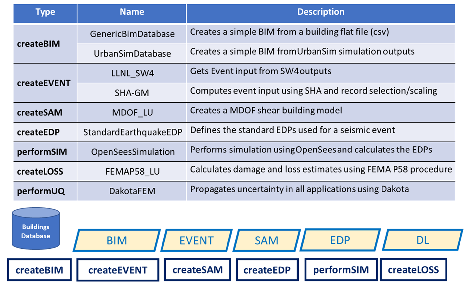
\includegraphics[width=1.0\textwidth, angle = 0]{editor/Figures/CompWorkflow.pdf}
    \caption{Computational workflow and registered applications for the San Francisco Bay Area Earthquake Scenario}
    \label{fig:intro_CompWorkflow}
\end{figure}

\paragraph{AI Applications} One of the key challenges for building regional hazard scenarios is creation of actual BIMs (Building Information Models) and SAMs (Structural Analysis Models) for the buildings in the region. To address this, the SimCenter has ongoing development to apply Artificial Intelligence (AI) methods to develop ``aiBIM'' and ``aiSAM'' applications. The ``aiBIM'' application utilizes visual imagery combined with other databases (e.g., parcel level tax data, LIDAR imagery, etc.) to develop a detailed database of buildings and their features. The ``aiSAM'' application translates BIM information into SAM to simulate the damaging effects of earthquakes, wind, and water inundation.
%\newline

\noindent This report has laid out the state of the art as seen by the authors of the respective sections as of the date of this report and how the SimCenter's current and future developments are aligned with these observations. The report thus serves not only as a state-of-the-art report for general consumption but also as a guiding document for the SimCenter. We hope that its contents find wide use and help focus research and software development needs in the NHERI community.
